\chapter{Discussion}
Please tell more about conclusion and how to the next work of this study.

\section{Annisa Fathoroni/1164067}
\subsection{Teori}
Penjelasan Tugas Harian 11 ( No 1-8 ).
\begin{enumerate}
\item Mengapa file suara harus dilakukan MFCC, dilengkapi dengan ilustrasi atau gambar.

Mel Frequency Cepstral Coefficients (MFCC) merupakan koefisien yang merepresentasikan audio. Sehingga diharuskannya melakukan MFCC kepada objek suara atau audio agar suara dapat berubah atau diubah ke dalam bentuk data matrix dimana telah dilakukan ekstraksi oleh MFCC kemudian direalisasikan sebagai data matrix.

\begin{itemize}
\item Ilustrasi Gambar:

\begin{figure}[!hbtp]
\centering
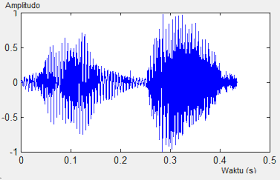
\includegraphics[scale=0.7]{figures/Chapter6AnnisaFathoroni1.png}
\caption{MFCC - Annisa Fathoroni}
\label{MFCC - Annisa Fathoroni}
\end{figure}

\end{itemize}

\item Konsep dasar Neural Network, dilengkapi dengan ilustrasi atau gambar.

Neural Network merupakan replika dari sistem syaraf yang terdapat pada sistem otak manu- sia. Dalam proses kerjanya, otak manusia disusun atas miliaran neuron dimana masing-masing neuron akan terhubung pada puluhan ribu neuron lain.
\begin{itemize}
\item Ilustrasi Gambar:

\begin{figure}[!hbtp]
\centering
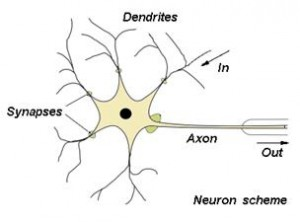
\includegraphics[scale=0.7]{figures/Chapter6AnnisaFathoroni2.jpg}
\caption{Konsep Dasar Neural Network - Annisa Fathoroni}
\label{Konsep Dasar Neural Network - Annisa Fathoroni}
\end{figure}

\end{itemize}

\item Konsep pembobotan Neural Network, dilengkapi dengan ilustrasi atau gambar.

Bobot merupakan suatu nilai yang mendefinisikan tingkat atau kepentingan hubungan antara suatu node dengan node yang lain. Semakin besar bobot  suatu hubungan menandakan semakin pentingnya hubungan kedua node tersebut. Bobot merupakan suatu hubungan berupa bilangan real maupun integer, tergantung dari jenis permasalahan dan model yang digunakan. Bobot-bobot tersebut bisa ditentukan untuk berada didalam interval tertentu. selama proses pelatihan, bobot tersebut dapat menyesuaikan dengan pola-pola input.

\begin{itemize}
\item Ilustrasi Gambar :

\begin{figure}[!hbtp]
\centering
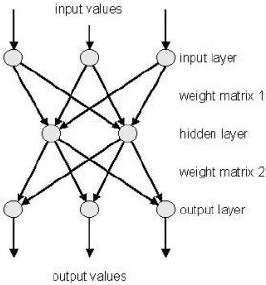
\includegraphics[scale=0.7]{figures/Chapter6AnnisaFathoroni3.jpg}
\caption{Konsep Pembobotan Neural Network - Annisa Fathoroni}
\label{Konsep Pembobotan Neural Network - Annisa Fathoroni}
\end{figure}

\end{itemize}

\item Konsep fungsi aktifasi dalam Neural Network, dilengkapi dengan ilustrasi atau gambar.
Operasi matematik yang dikenakan pada sinyal output y. Sehingga fungsi ini akan digunakan untuk pengaktifan dan juga penonaktifan neuron.
\begin{itemize}
\item Dalam konsep fungsi aktivasi Neuron Network terdapat beberapa jenis:
\begin{itemize}
\item Fungsi Undak Biner Hard Limit ( Menkonversi nilai masukan dari suatu variabel )
\item Fungsi Undak Biner Threshold ( Menggunakan nilai ambang 0 sebagai batas eksekusil )
\item Fungsi Bipolar Symetric Hard Limit ( Mempunyai keluaran bernilai 1 dan 0 )
\item Fungsi Bipolar Threshold ( Mempunyai keluaran bernilai 1, 0 atau -1 )

\item Ilustrasi Gambar:

\begin{figure}[!hbtp]
\centering
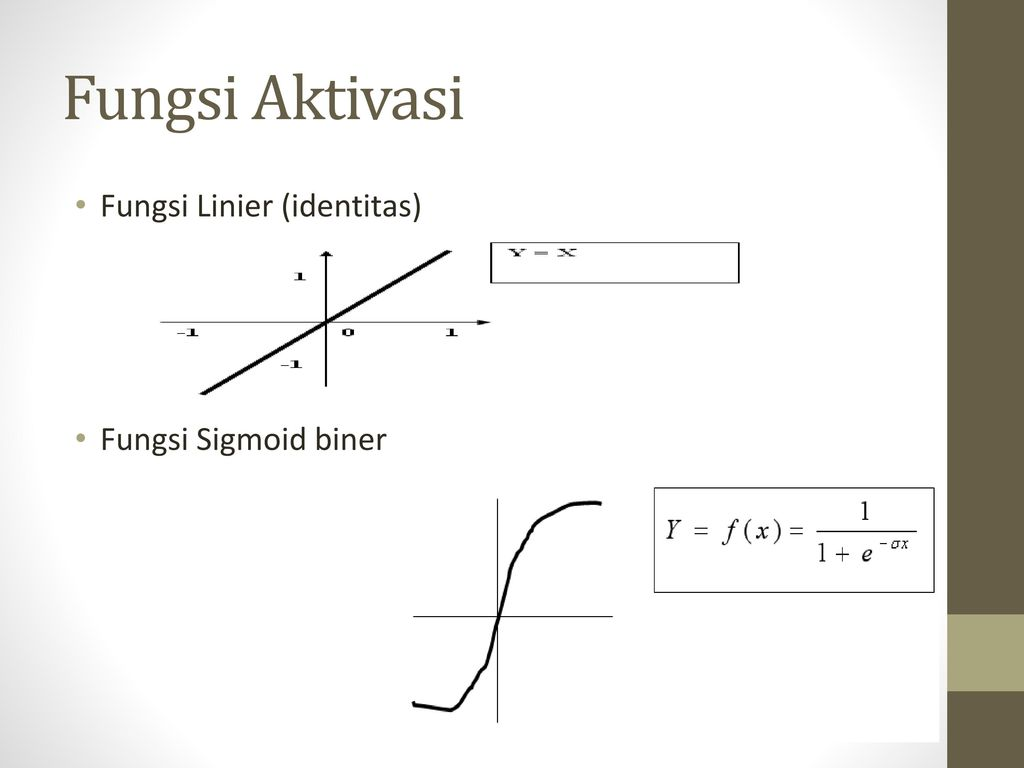
\includegraphics[scale=0.7]{figures/Chapter6AnnisaFathoroni4.jpg}
\caption{Konsep Fungsi Aktifasi - Annisa Fathoroni}
\label{Konsep Fungsi Aktivasi - Annisa Fathoroni}
\end{figure}

\end{itemize}
\end{itemize}

\item Cara membaca hasil plot dari MFCC, dilengkapi dengan ilustrasi atau gambar.

Penjelasan Cara Membaca Hasil Plot Dari MFCC :
\begin{itemize}
\item Ilustrasi Gambar :
\begin{figure}[!hbtp]
\centering
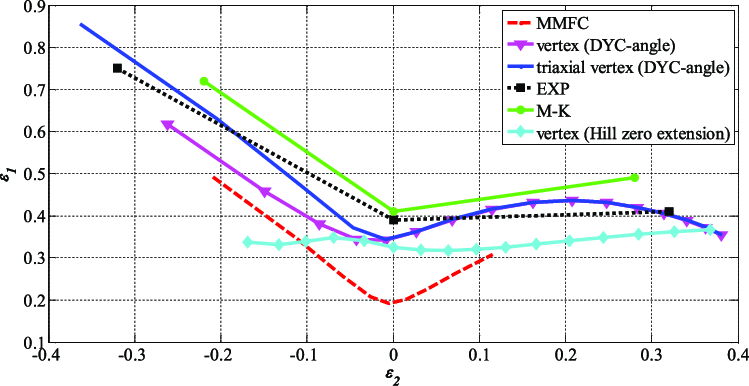
\includegraphics[scale=0.4]{figures/Chapter6AnnisaFathoroni5.png}
\caption{Plot MFCC - Annisa Fathoroni}
\label{Plot MFCC - Annisa Fathoroni}
\end{figure}

\end{itemize}

\item Apa itu One-Hot Encoding, dilengkapi dengan ilustrasi atau gambar.


One-Hot Encoding adalah sekelompok bit yang kombinasi hukumnya hanya terdiri dari bit dengan bit tinggi (1) dan bit lainnya rendah (0). Implementasi serupa di mana semua bit '1' kecuali satu '0' kadang-kadang disebut one-cold. Dalam statistik, variabel dummy mewakili teknik serupa untuk mewakili data kategorikal.
\begin{itemize}
\item Ilustrasi Gambar:

\begin{figure}[!hbtp]
\centering
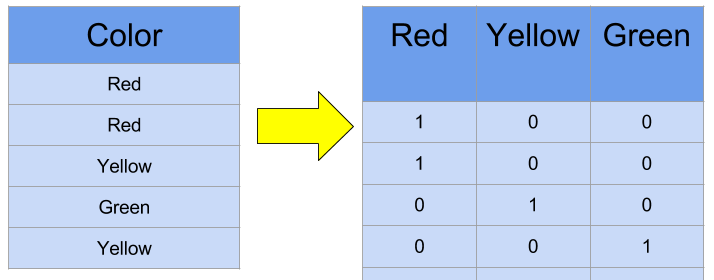
\includegraphics[scale=0.4]{figures/Chapter6AnnisaFathoroni6.png}
\caption{One-Hot Encoding - Annisa Fathoroni}
\label{One-Hot Encoding - Annisa Fathoroni}
\end{figure}

\end{itemize}

\item Fungsi dari np.unique dan to.categorical, dilengkapi dengan ilustrasi atau gambar.
\begin{enumerate}
\item np.unique:

Berfungsi untuk menemukan elemen unik array. Ada tiga output opsional selain elemen unik:

\begin{itemize}
\item Indeks array input yang memberikan nilai unik
\item Indeks array unik yang merekonstruksi array input
\item Berapa kali setiap nilai unik muncul dalam array input
\end{itemize}

\item Ilustrasi Gambar :

\begin{figure}[!hbtp]
\centering
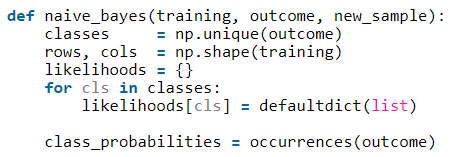
\includegraphics[scale=0.7]{figures/Chapter6AnnisaFathoroni7-1.png}
\caption{np.unique - Annisa Fathoroni}
\label{np.unique - Annisa Fathoroni}
\end{figure}

\item to.categorical:

Berfungsi untuk mengubah vektor kelas yang berupa integer menjadi matriks kelas biner.

\begin{itemize}
\item Ilustrasi Gambar :

\begin{figure}[!hbtp]
\centering
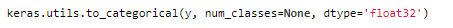
\includegraphics[scale=0.7]{figures/Chapter6AnnisaFathoroni7-2.png}
\caption{to.categorical - Annisa Fathoroni}
\label{to.categorical - Annisa Fathoroni}
\end{figure}

\end{itemize}
\end{enumerate}

\item Fungsi dari Sequential, dilengkapi dengan ilustrasi atau gambar.
Sebuah jenis model yang digunakan dalam perhitungan ataupun code program yang direalisasikan.
\begin{itemize}
\item Ilustrasi Gambar:

\begin{figure}[!hbtp]
\centering
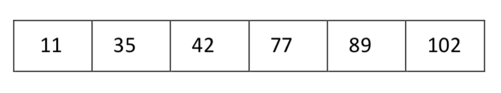
\includegraphics[scale=0.7]{figures/Chapter6AnnisaFathoroni8.png}
\caption{Sequential - Annisa Fathoroni}
\label{Sequential - Annisa Fathoroni}
\end{figure}

\end{itemize}
\end{enumerate}

\section{Tasya Wiendhyra / 1164086}
\subsection{Teori}
\begin{enumerate}
\item Kenapa file suara harus di lakukan MFCC. dilengkapi dengan ilustrasi atau gambar. \\
\par Nilai-nilai MFCC meniru pendengaran manusia dan mereka biasanya digunakan dalam aplikasi pengenalan suara serta genre musik
deteksi. Nilai-nilai MFCC ini akan dimasukkan langsung ke jaringan saraf.Agar dapat diubah menjadi bentuk vektor, dan dapat digunakan pada machine learning. Disebabkan machine learning hanya mengerti bilangan vektor saja.\\
Ilustrasinya, Ketika ingin menggunakan file suara dalam machine learning, misalnya untuk melihat jam. Machine learning tidak memahami rekaman suara melainkan vektor. Maka rekaman tersebut akan diubah kedalam bentuk vektor kemudian vektor akan menyesuaikan dengan kata kata yang sudah disediakan. Jika cocok maka akan mengembalikan waktu yang diinginkan

\item Konsep dasar neural network dilengkapi dengan ilustrasi atau gambar
\par Neural Network ini terinspirasi dari jaringan saraf otak manusia. Dimana setiap neuron terhubung ke setiap neuron di lapisan berikutnya. Lapisan pertama menerima input dan lapisan terakhir memberikan keluaran. Struktur jaringan, yang berarti jumlah neuron dan koneksinya, diputuskan sebelumnya dan tidak dapat berubah, setidaknya tidak selama training. Juga, setiap input harus memiliki jumlah nilai yang sama. Ini berarti bahwa gambar, misalnya, mungkin perlu diubah ukurannya agar sesuai dengan jumlah neuron input.\\

Ilustrasinya. misalkan kita ingin encode sebuah kalimat yaitu "what time is it" kemudian Anda menginisialisasi lapisan jaringan Anda dan hidden statel. Bentuk dan dimensi hidden state akan tergantung pada bentuk dan dimensi jaringan saraf berulang Anda. Kemudian Anda mengulangi input Anda, meneruskan kata danhidden state ke NN. NN mengembalikan output dan kondisi tersembunyi yang dimodifikasi. Anda terus mengulang sampai Anda kehabisan kata-kata. Terakhir Anda melewatkan output ke layer feedforward, dan itu mengembalikan prediksi. Bahwa kita ingin mengetahui pukul berapa sekarang.

\item Konsep pembobotan dalam neural network.dilengkapi dengan ilustrasi atau gambar
\par Bobot mewakili kekuatan koneksi antar unit. Jika bobot dari node 1 ke node 2 memiliki besaran lebih besar, itu berarti bahwa neuron 1 memiliki pengaruh lebih besar terhadap neuron. 2. Bobot penting untuk nilai input. Bobot mendekati nol berarti mengubah input ini tidak akan mengubah output. Bobot negatif berarti meningkatkan input ini akan mengurangi output. Bobot menentukan seberapa besar pengaruh input terhadap output. Seperti contoh berikut :
\begin{figure}[ht]
\centering
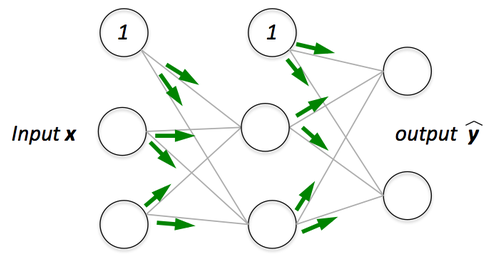
\includegraphics[scale=0.5]{figures/chapter6tasya2.png}
\caption{Contoh Pembobotan Neural Network Tasya}
\label{Teori}
\end{figure}

\item Konsep fungsi aktifasi dalam neural network. dilengkapi dengan ilustrasi atau gambar
\par Fungsi aktivasi digunakan untuk memperkenalkan non-linearitas ke jaringan saraf. Ini menekan nilai dalam rentang yang lebih kecil yaitu. fungsi aktivasi Sigmoid memeras nilai antara rentang 0 hingga 1. Ada banyak fungsi aktivasi yang digunakan dalam industri pembelajaran yang dalam dan ReLU, SeLU dan TanH lebih disukai daripada fungsi aktivasi sigmoid. Ilustrasinya, ketika fungsi aktivasi linier, jaringan saraf dua lapis mampu mendekati hampir semua fungsi. Namun, jika fungsi aktivasi identik dengan fungsi aktivasi F (X) = X), properti ini tidak puas, dan jika MLP menggunakan fungsi aktivasi yang sama, seluruh jaringan setara dengan jaringan saraf lapis tunggal.

\item Cara membaca hasil plot dari MFCC,dilengkapi dengan ilustrasi atau gambar\\
Berikut merupakan hasil plot dari rekaman suara :
\begin{figure}[ht]
\centering
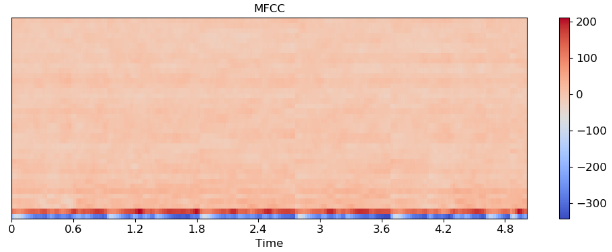
\includegraphics[scale=0.5]{figures/chapter6tasya1.png}
\caption{Cara Membaca Hasil Plot MFCC Tasya}
\label{Teori}
\end{figure}
Dari gambar tersebut dapat diketahui :\\
\begin{itemize}
\item Terdapat 2 dimensi yaitu x sebagai waktu, dan y sebagai power atau desibel.
\item Dapat dilihat bahwa jika berwarna biru maka power dari suara tersebut rendah, dan jika merah power dari suara tersebut tinggi
\item Dibagian atas terdapat warna merah pudar yang menandakan bahwa tidak ada suara sama sekali dalam jangkauan tersebut.
\end{itemize}

\item Jelaskan apa itu one-hot encoding,dilengkapi dengan ilustrasi kode dan atau gambar.
\par One-hot encoding adalah representasi variabel kategorikal sebagai vektor biner. Mengharuskan nilai kategorikal dipetakan ke nilai integer. Kemudian, setiap nilai integer direpresentasikan sebagai vektor biner yang semuanya bernilai nol kecuali indeks integer, yang ditandai dengan 1.
\begin{figure}[ht]
\centering
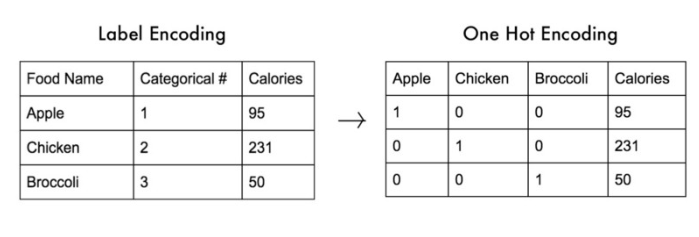
\includegraphics[scale=0.5]{figures/chapter6tasya3.png}
\caption{One Hot Encoding Tasya}
\label{Teori}
\end{figure}

\item fungsi dari np/.unique dan to categorical dalam kode program,dilengkapi dengan ilustrasi atau gambar.\\
Untuk np unique fungsinya yaitu menemukan elemen unik array. Mengembalikan elemen unik array yang diurutkan. Ada tiga output opsional selain elemen unik:\\
\begin{itemize}
\item Indeks array input yang memberikan nilai unik
\item Indeks array unik yang merekonstruksi array input
\item Berapa kali setiap nilai unik muncul dalam array input.
\end{itemize}
\begin{figure}[ht]
\centering
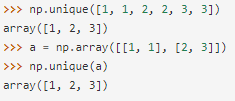
\includegraphics[scale=0.5]{figures/chapter6tasya4.png}
\caption{Numpy Unique Tasya}
\label{Teori}
\end{figure}

Untuk  To Categorical fungsinya untuk mengubah vektor kelas (integer) ke matriks kelas biner.
\begin{figure}[ht]
\centering
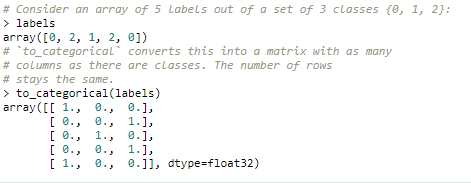
\includegraphics[scale=0.5]{figures/chapter6tasya5.png}
\caption{To Categorical Tasya}
\label{Teori}
\end{figure}

\item Fungsi dari Sequential dalam kode program,dilengkapi dengan ilustrasi atau gambar.\\
Sequential berfungsi sebagai tumpukan linear lapisan. COntohnya sebagai berikut :
\begin{figure}[ht]
\centering
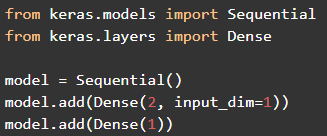
\includegraphics[scale=0.5]{figures/chapter6tasya6.png}
\caption{Sequential Tasya}
\label{Teori}
\end{figure}
\end{enumerate}
